\documentclass{article}
\usepackage{arxiv}

\usepackage[utf8]{inputenc}
\usepackage[english, russian]{babel}
\usepackage[T1]{fontenc}
\usepackage{url}
\usepackage{booktabs}
\usepackage{amsfonts}
\usepackage{nicefrac}
\usepackage{microtype}
\usepackage{lipsum}
\usepackage{graphicx}
\usepackage{natbib}
\usepackage{doi}



\title{Декодирования сигналов головного мозга в аудиоданные}

\author{ Набиев Мухаммадшариф \\
        Кафедра интеллектуальных систем\\
	МФТИ\\
	\texttt{nabiev.mf@phystech} \\
	\And
	Северилов Павел \\
	Кафедра интеллектульных систем\\
	МФТИ\\
	\texttt{pseverilov@gmail.com} \\
	%% \AND
	%% Coauthor \\
	%% Affiliation \\
	%% Address \\
	%% \texttt{email} \\
	%% \And
	%% Coauthor \\
	%% Affiliation \\
	%% Address \\
	%% \texttt{email} \\
	%% \And
	%% Coauthor \\
	%% Affiliation \\
	%% Address \\
	%% \texttt{email} \\
}
\date{}

\renewcommand{\shorttitle}{\textit{arXiv} Template}

%%% Add PDF metadata to help others organize their library
%%% Once the PDF is generated, you can check the metadata with
%%% $ pdfinfo template.pdf
\hypersetup{
pdftitle={Декодирования сигналов головного мозга в аудиоданные},
pdfsubject={q-bio.NC, q-bio.QM},
pdfauthor={Набиев Мухаммадшариф, Северилов Павел},
pdfkeywords={First keyword, Second keyword, More},
}

\begin{document}
\maketitle

\begin{abstract}
  В данной работе исследуется проблема декодирования сигналов головного мозга в аудиосигналы с использованием физически-информированных методов получения эмбеддингов сигналов. Предлагается решить задачу классификации стимулов по соответствующим сегментам аудиоданных. Под стимулом понимается аудиосигнал, который вызвал активность мозга, соответствующая ЭЭГ-сигналу. Данные для задачи представляют собой 668 пар вида ЭЭГ-стимул общей продолжительностью стимулов 9431 минута. В качестве метрики для выбора оптимальной модели используется F1-мера. В данной работе предлагается исследовать передовые методы машинного обучения, которые учитывают физические принципы, с целью улучшения качества обработки аудиосигналов и повышения точности их декодирования. Полученные результаты имеют важное значение для развития интерфейсов мозг-компьютер и понимания принципов обработки аудиосигналов человеческим мозгом.

\end{abstract}


\keywords{auditory EEG decoding \and natural speech processing \and EEG}

\section{Введение} 
    \par 
    Слух, одно из наиболее важных человеческих чувств, играет решающую роль в нашем повседневном взаимодействии с окружающим миром. Однако многие люди со всего мира сталкиваются с проблемами слуха, которые могут серьезно ограничить их способность воспринимать звуки окружающей среды. В свете этих проблем возникает интерес к исследованию взаимосвязи между звуком и мозговыми сигналами. В данной области выделена задача декодирования мозговых сигналов в аудиоданные. 
    \par 
    Задачу декодирования можно поставить двумя способами: классификация и регрессия. В данной работе мы сконцентрируемся на задаче классификации. Требуется решить задачу классификации в парадигме match-mismatch, когда на вход подается ЭЭГ сигнал и 5 стимулов, из которых только один соответствует сигналу. Под стимулом подразумевается сегмент аудио, который стимулировал сигнал в мозгу субъекта. 
    \par 
    Существует базовое решение этой задачи, использующее dilated convolutional network~\citep{Accou2021ModelingTR}. Оно имеет следующую архитектуру(Рис.~\ref{model}).
    \begin{figure}
	\centering
	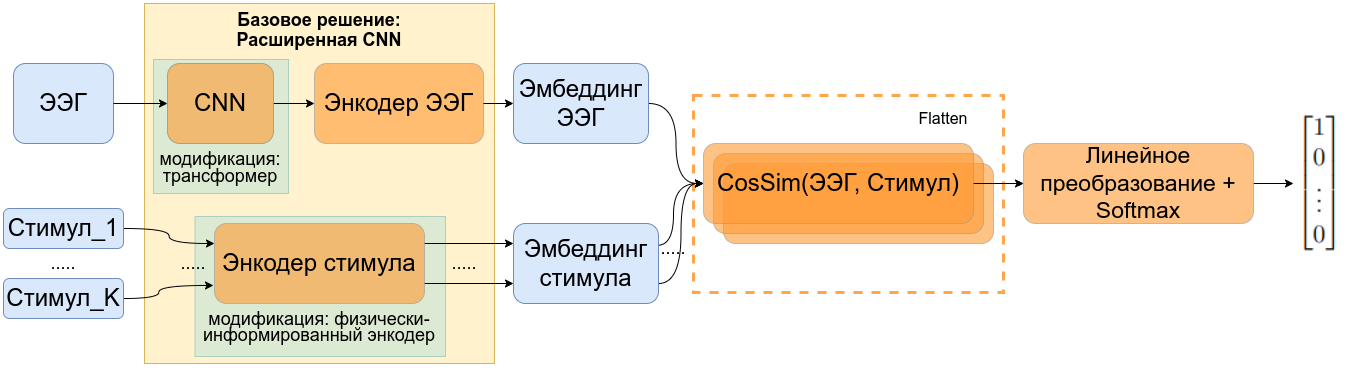
\includegraphics[width=1\textwidth]{model_architecture.png}
	\caption{Архитектура используемой модели. Базовое решение в качестве энкодера использует dilated convolutional network. В латентном пространстве считаются близости представлений, тем самым определяется наибольшое вероятное совпадение.}
	\label{model}
    \end{figure}
    В начале используется сверточный слой с 8 фильтрами для объединения данных из всех каналов ЭЭГ. Далее $N$ dilated свёрток с размером ядра K применяются к выходу первого слоя и к 5 стимулам. Для каждого слоя $L_n$ dilation factor рассчитывается, как $K^{n - 1}$, которое взято из статьи \citep{vandenoord16_ssw}, для того, чтобы минимизировать количество параметров. На выходе каждой свертки применяется функция активации ReLU. Затем вычисляется косинусный коэффициент между представлением ЭЭГ и представлениями стимулов. Наконец, линейный слой с сигмоидой используя эти коэффициенты классифицирует стимулы. 
    \par 
    Известна модификация базового решения с использованием Multi-Head Attentionи и GRU~\citep{multihead-gru}. Дополнительно авторы генерируют также и спектрограмму для получения дополнительных признаков, как, например, частота. Также в отличие от базового решения стимулы и спектрограммы проходят через GRU, а уже пото подаются на вход в dilated convolutional блоки. 
    \par 
    Решению задачи декодирования в постановке регрессии посвящена статья~\cite{piao2023happyquokka}. Авторами была предложена модель Pre-LLN FFT, основанная на модели Feed-Forward Transformer(FFT) network из \citep{ren2019fastspeech}. За счет модификации FFT и добавления global conditioner~\citep{vandenoord16_ssw} и нормализации пред-слоя~\citet{xiong2020layer}, авторы добились улучшения коэффициента корелляции Пирсона по сравнению с базовым решением использовавшим Very Large Augmented Auditory Inference(VLAAI)~\citep{vlaai}. 
    
    Предлагается воспользоваться физическими принципами при решении задачи классификации. А именно, по стимулам сгенерировать mel-спектрограммы, а также воспользоваться Self-Attention-ом для учета дополнительных деталей голоса из стимулов и спектрограмм. 
    
\section{Данные}
    Были использованы данные SparrKULee~\citep{K3VSND_2023}. Данные состоят из записей ЭЭГ 85 молодых людей (18 - 30 лет) с хорошим слухом, каждый из которых слушал естественную речь на протяжении 90-150 минут. 


\section{Постановка задачи}
    Сигналы ЭЭГ представляет собой матрицу $\mathbf{X}=[\mathbf{x}^{\mathsf{T}}_1,...,\mathbf{x}^{\mathsf{T}}_m]^{\mathsf{T}} \in \mathbb{R}^{n \times m}$, где $n$-количество каналов, а  $m$-время. Обозначим стимулы и их метки, как $(\mathbf{s}_1, y_1), \dots, (\mathbf{s}_5, y_5) \in \mathbb{R}^{1 \times m} \times \{ 0, 1\}$ . Требуется по имеющимся $\mathbf{X}, \mathbf{s}_1, \dots, \mathbf{s}_5$ и $\mathbf{y} = [y_1, \dots, y_5]^T$ предсказать вероятность для каждого стимула $\mathbf{s}_k$. Допустим, что модель из $\mathbf{F} \subset \mathfrak{F}$, $\mathfrak{F}$-параметрическое множество моделей. Тогда задача сводится к минимизации Cross-Entropy Loss:
    $$CE = - \sum_{k=1}^5 y_k \log (\mathbf{F}(\mathbf{X}, \mathbf{s}_k))$$.

\subsection{Описание модели}
    На входе сигналы ЭЭГ проходят через 1D сверточный слой с 8 фильтрами и ядром $1 \times 1$ для пространственной связки каналов и уменьшения размерности. $\tilde{\mathbf{X}} = \mathrm{Conv}(\mathbf{X}, K_1)$, где $K_1$ ядро слоя. Матрица $\tilde{\mathbf{X}}$ является двумерной и её размерность составляет $8 \times m$. Преобразованные сигналы ЭЭГ проходят через N dilated сверточных слоев с ядром $K_2$ размерностью $3 \times 3$ и 16 фильтрами. На слое $L_p$ dilation factor возьмем равным $K^{p-1}$. В итоге получим итоговое представление ЭЭГ в виде матрицы $16 \times m'$. Через этот же сверточный слой пройдут и стимулы $\mathbf{s}_1, \dots, \mathbf{s}_5$ и каждый из них также будет отображен в латентое пространство $M_{16\times m'}(\mathbb{R})$ - пространство вещественных матрица размера $16 \times m'$. Получив представления в латентном пространстве высчитываются косинусные коэффициенты $$C_k = \mathrm{CosSim}(\mathbf{X}_{emb}, \mathbf{s}_{emb}),$$ 
    где скалярное произведение производится по столбцам. Каждая матрица $C_k$ размерностью $16 \times 16$ подается на вход в линейной слой $c_k = Linear(C_k)$. В итоге по вектору $[c_1, \dots, c_5]^T$ вычисляется $\mathrm{Softmax}$, по значениям которой и определяется какой стимул является истинным. 

\section{Вычислительный эксперимент}
    Эксперимент будет проверяться на данных~\citep{K3VSND_2023}. Данные представляют собой выборку из 85 человек. Все участники прослушали 6, 7, 8 или 10 стимулов, каждая из которых имеет примерную продолжительность 15 мин. После прослушивания участников спрашивали про содержания аудиофрагмента. Это было с целью мотивировать участников обращать внимания во время прослушивания.

    Стимулы были разделены на следующие категории:

    \begin{itemize}
        \item Референсные аудиокниги
        \item Аудиокниги для детей и взрослых. Если длина превышала 15 мин, то аудиокнига делилась на части
        \item Аудиокниги с шумом
        \item Подкасты про ответы на научные вопросы
        \item Подкасты с видео
    \end{itemize}

    Также отметим, согласно авторам, что частота дискретизации ЭЭГ и стимулов была занижена до 64 Гц.

    Обработанные стимулы представляют собой огибающую кривую сигнала аудиофрагмента. 
    \begin{figure}[h]
	\centering
	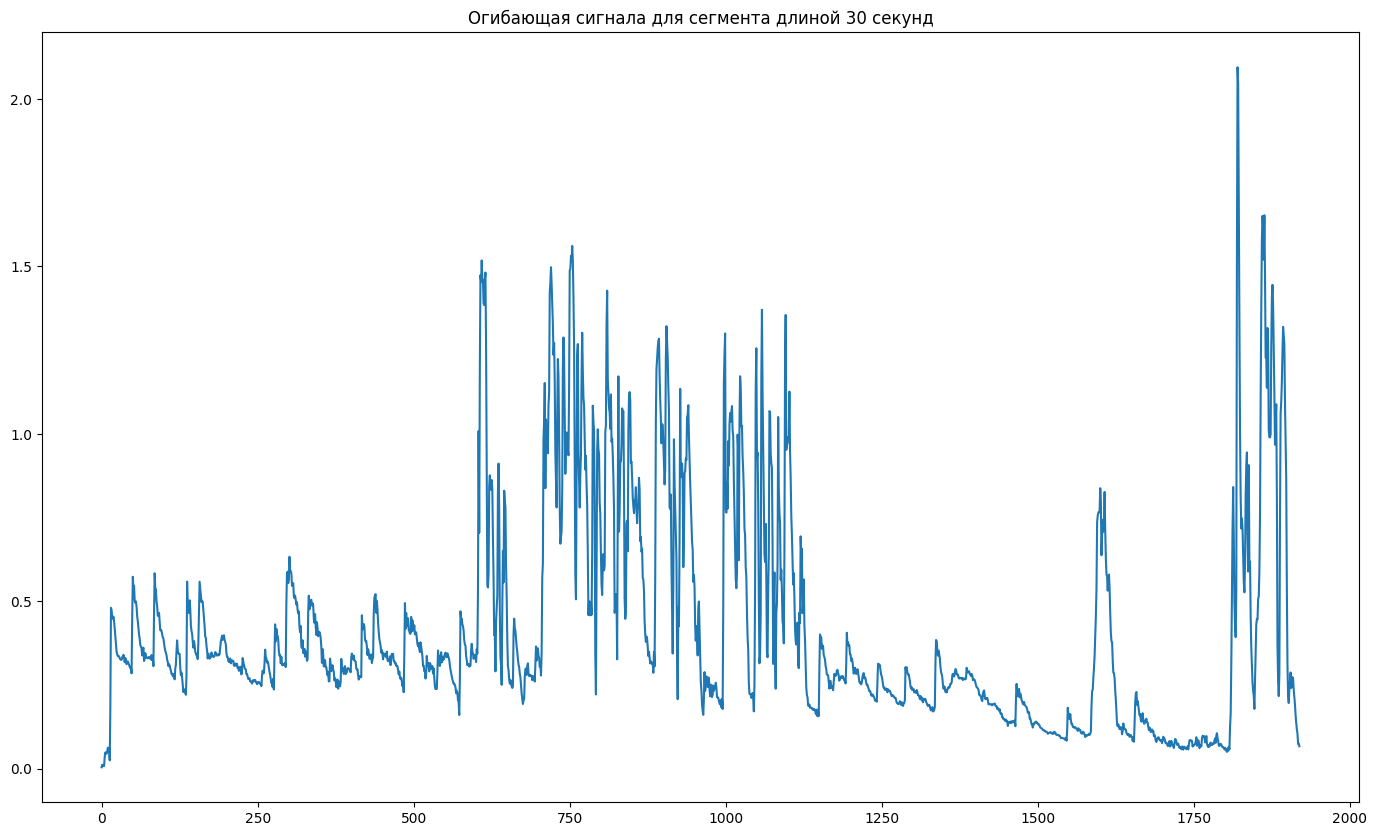
\includegraphics[width=0.7\textwidth]{envelope_example.png}
	\caption{Пример огибающей сигнала}
	\label{dilated_conv}
    \end{figure}

    Всего в имеем 665 пар ЭЭГ-стимул. Данные были разбиты на тренировочную, валидационную и тестовую части в соотношении $80\% : 10\%  : 10\%$. 
    
    На вход модели подаются ЭЭГ и $k$ стимулов. Из поданных $k$ стимулов один является истинным, соответствующему ЭЭГ, а остальные ложные. Энкодеры модели отображают ЭЭГ сигнал и стимулы в латентное пространство. В этом пространстве вычисляется косинусный коэффициент пар (преобразованный ЭЭГ, преобразованный $k$-й стимул). Качество измеряем с помощью F1-меры. 

    Эксперимент проводился на $10$ эпохах, а размер батча составлял 16 объектов, количество ложных стимулов $k=4$. 

    Измерения на маленькой части данных. Результаты приведены на графике~\ref{res} 
    \begin{figure}[h]
	\centering
	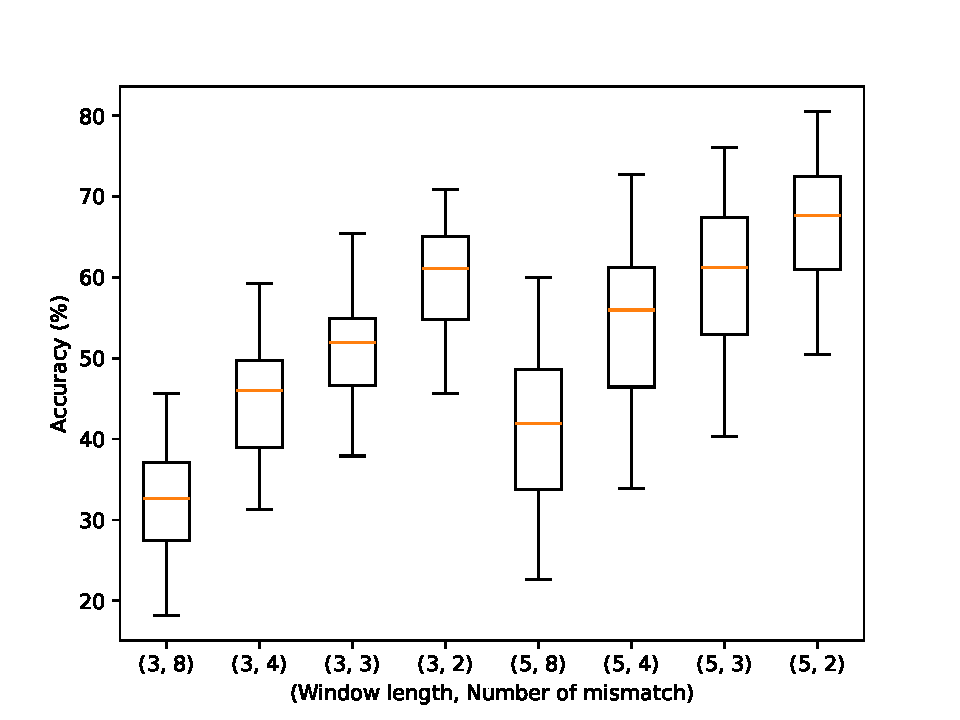
\includegraphics[width=0.7\textwidth]{boxplot_dilated_conv.pdf}
	\caption{Зависимость точности от размера окна и количества ложных стимулов}
	\label{res}
    \end{figure}
    
    
\bibliographystyle{plain}
\bibliography{Nabiev2024SignalToAudio}

\end{document}